% =========================================================
% Bounds, Suprema, Infima + Table + Figure
% =========================================================

\subsection{Bounds and Extremal Values}

\begin{figure}[h]
\centering
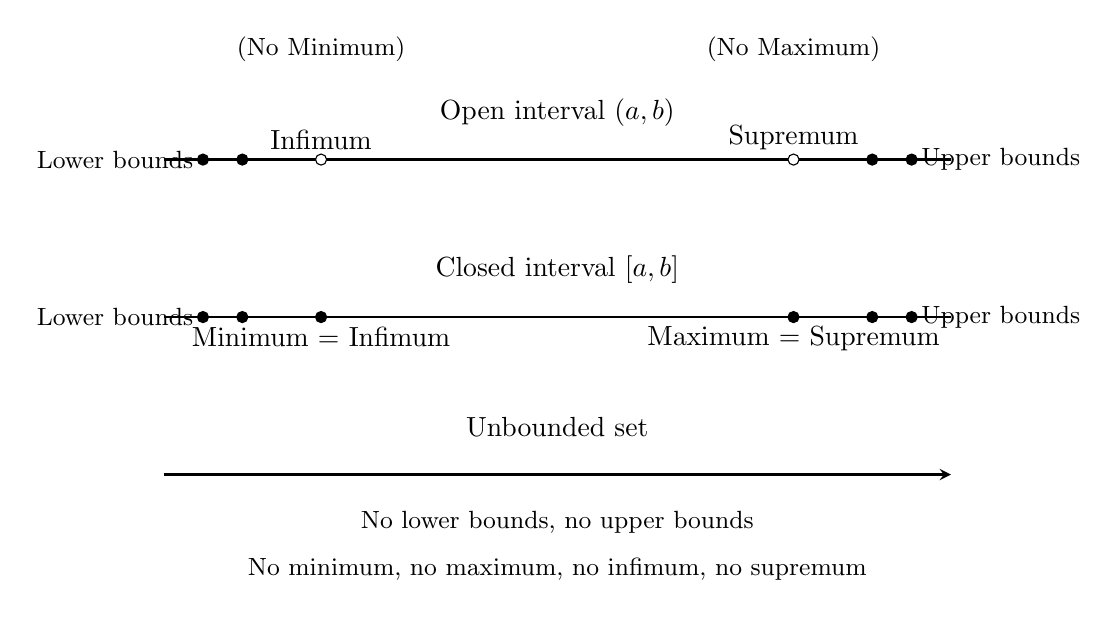
\begin{tikzpicture}[x=1cm,y=1cm,>=stealth]

% =====================
% OPEN INTERVAL (a,b)
% =====================
\draw[thick] (-5,3) -- (5,3);
\draw[fill=white] (-3,3) circle (2pt);
\draw[fill=white] (3,3) circle (2pt);

\node at (0,3.6) {Open interval $(a,b)$};

% Infimum / Supremum
\node[above] at (-3,3) {Infimum};
\node[above] at (3,3) {Supremum};
\node at (-3,4.4) {\small (No Minimum)};
\node at (3,4.4) {\small (No Maximum)};

% Lower bounds
\draw[fill] (-4.5,3) circle (2pt);
\draw[fill] (-4,3) circle (2pt);
\node[left] at (-4.5,3) {\small Lower bounds};

% Upper bounds
\draw[fill] (4,3) circle (2pt);
\draw[fill] (4.5,3) circle (2pt);
\node[right] at (4.5,3) {\small Upper bounds};

% =====================
% CLOSED INTERVAL [a,b]
% =====================
\draw[thick] (-5,1) -- (5,1);
\draw[fill] (-3,1) circle (2pt);
\draw[fill] (3,1) circle (2pt);

\node at (0,1.6) {Closed interval $[a,b]$};

% Min / Max
\node[below] at (-3,1) {Minimum = Infimum};
\node[below] at (3,1) {Maximum = Supremum};

% Lower bounds
\draw[fill] (-4.5,1) circle (2pt);
\draw[fill] (-4,1) circle (2pt);
\node[left] at (-4.5,1) {\small Lower bounds};

% Upper bounds
\draw[fill] (4,1) circle (2pt);
\draw[fill] (4.5,1) circle (2pt);
\node[right] at (4.5,1) {\small Upper bounds};

% =====================
% UNBOUNDED SET
% =====================
\draw[thick,->] (-5,-1) -- (5,-1);

\node at (0,-0.4) {Unbounded set};

\node at (0,-1.6)
{\small No lower bounds, no upper bounds};

\node at (0,-2.2)
{\small No minimum, no maximum, no infimum, no supremum};

\end{tikzpicture}
\caption{Bounds, extrema, infimum, and supremum for subsets of $\mathbb{R}$.}
\end{figure}

\begin{center}
\begin{tabular}{|p{4cm}|p{9cm}|}
\hline
\textbf{Concept} & \textbf{What you must show} \\
\hline

Upper bound &
To show that $u$ is an upper bound for $A$, prove that
\[
\forall a \in A,\quad a \le u.
\]
\\ \hline

Supremum &
To show that $u=\sup A$, prove:
\begin{itemize}
\item $u$ is an upper bound for $A$, and
\item every upper bound $v$ of $A$ satisfies $u \le v$.
\end{itemize}
\\ \hline

Bounded above &
To show that $A$ is bounded above, prove that
there exists at least one upper bound for $A$.
\\ \hline

Maximum &
To show that $m=\max A$, prove that $m$ is an upper bound for $A$
and that $m \in A$.
\\ \hline

\end{tabular}
\end{center}

\begin{definition}[Upper Bound]
Let $A \subseteq \mathbb{R}$.
A number $u \in \mathbb{R}$ is an \emph{upper bound} for $A$ if
\[
\forall a \in A,\quad a \le u.
\]
\end{definition}

\begin{definition}[Lower Bound]
Let $A \subseteq \mathbb{R}$.
A number $\ell \in \mathbb{R}$ is a \emph{lower bound} for $A$ if
\[
\forall a \in A,\quad \ell \le a.
\]
\end{definition}

\begin{definition}[Bounded Above / Below]
A set $A \subseteq \mathbb{R}$ is said to be:
\begin{itemize}
\item \emph{bounded above} if it has at least one upper bound;
\item \emph{bounded below} if it has at least one lower bound;
\item \emph{bounded} if it is both bounded above and bounded below.
\end{itemize}
\end{definition}

\begin{definition}[Supremum (Least Upper Bound)]
Let $A \subseteq \mathbb{R}$ be nonempty and bounded above.
A number $s \in \mathbb{R}$ is the \emph{supremum} of $A$, written $s=\sup A$, if:
\begin{enumerate}
\item $s$ is an upper bound for $A$, and
\item if $u$ is any upper bound for $A$, then $s \le u$.
\end{enumerate}
\end{definition}

\begin{definition}[Infimum (Greatest Lower Bound)]
Let $A \subseteq \mathbb{R}$ be nonempty and bounded below.
A number $i \in \mathbb{R}$ is the \emph{infimum} of $A$, written $i=\inf A$, if:
\begin{enumerate}
\item $i$ is a lower bound for $A$, and
\item if $\ell$ is any lower bound for $A$, then $\ell \le i$.
\end{enumerate}
\end{definition}

\begin{definition}[Maximum]
Let $A \subseteq \mathbb{R}$.
A number $m \in A$ is a \emph{maximum} of $A$, written $m=\max A$, if
\[
\forall a \in A,\quad a \le m.
\]
\end{definition}

\begin{definition}[Minimum]
Let $A \subseteq \mathbb{R}$.
A number $m \in A$ is a \emph{minimum} of $A$, written $m=\min A$, if
\[
\forall a \in A,\quad m \le a.
\]
\end{definition}

\subsubsection{Epsilon Characterizations}

\begin{definition}[Supremum — $\varepsilon$ Definition]
Let $A \subseteq \mathbb{R}$ be nonempty and bounded above, and let $s \in \mathbb{R}$.
Then $s = \sup A$ if and only if:
\begin{enumerate}
\item $s$ is an upper bound for $A$, and
\item for every $\varepsilon > 0$, there exists $a \in A$ such that
\[
s - \varepsilon < a.
\]
\end{enumerate}
\end{definition}

\begin{definition}[Infimum — $\varepsilon$ Definition]
Let $A \subseteq \mathbb{R}$ be nonempty and bounded below, and let $i \in \mathbb{R}$.
Then $i = \inf A$ if and only if:
\begin{enumerate}
\item $i$ is a lower bound for $A$, and
\item for every $\varepsilon > 0$, there exists $a \in A$ such that
\[
a < i + \varepsilon.
\]
\end{enumerate}
\end{definition}

\subsubsection{Directional $\varepsilon$-Characterizations}

\paragraph{Supremum: $\varepsilon$-approximation from below}
If $s=\sup A$, then
\[
\forall \varepsilon>0,\ \exists a\in A \ \text{such that}\ s-\varepsilon < a \le s.
\]

\paragraph{Infimum: $\varepsilon$-approximation from above}
If $i=\inf A$, then
\[
\forall \varepsilon>0,\ \exists a\in A \ \text{such that}\ i \le a < i+\varepsilon.
\]

\medskip


